% Archivo actualizado a partir del aporte original de Landy Fuertes.
% Se conservan sus seis roles originales y sus ocho perspectivas sin reescritura.
% El bloque repetido se conserva en el archivo de respaldo original,
% no se integra aqui para evitar etiquetas LaTeX duplicadas.
% ==============================================================================
% APORTE DE LANDY FUERTES - SECCIÓN 2 (MATRIZ) Y SECCIÓN 3 (CONTEXTO)
% ==============================================================================
% ==============================================================================
% APORTE INDIVIDUAL: FUERTES CALVO LANDY LORENA
% SECCIÓN: PARTES INTERESADAS (8 ROLES PROPUESTOS) Y CONTEXTO DEL SISTEMA (DENTITECH)
% ==============================================================================
\section{Partes Interesadas y Contexto del Sistema}

\subsection{Identificaci\'on y Caracterizaci\'on de Partes Interesadas}

Conforme a la norma ISO/IEC/IEEE 29148:2018 \cite{iso29148}, la especificaci\'on rigurosa de requisitos demanda identificar previamente a las partes interesadas que interact\'uan con el sistema o reciben impacto de su operaci\'on en la \textbf{Cl\'inica Odontol\'ogica Medicus}, ubicada en el sector Cooperativa Jet de la ciudad de Quevedo, provincia de Los R\'ios, Ecuador. Para garantizar el cumplimiento de confidencialidad establecido en la Ley Org\'anica de Protecci\'on de Datos Personales (LOPDP) \cite{lopdp2021}, los actores se caracterizan exclusivamente por su rol organizacional, sin registrar identidades personales.

La Tabla~\ref{tab:partes_interesadas} detalla los ocho roles propuestos para la operaci\'on de la Cl\'inica Odontol\'ogica Medicus, su inter\'es principal respecto al sistema \textbf{DentiTech}, su grado de influencia sobre las decisiones del proyecto, su disponibilidad estimada para las sesiones de elicitaci\'on y la estrategia de participaci\'on asignada.

\begin{table}[htbp]
\centering
\caption{Caracterizaci\'on de las partes interesadas de la Cl\'inica Odontol\'ogica Medicus.}
\label{tab:partes_interesadas}
\scriptsize
\setlength{\tabcolsep}{4pt}
\renewcommand{\arraystretch}{1.25}
\begin{tabularx}{\textwidth}{|p{2.2cm}|X|c|c|p{1.8cm}|X|}
\hline
\textbf{Rol} & \textbf{Inter\'es Principal en DentiTech} & \textbf{Influencia} & \textbf{Inter\'es} & \textbf{Disponibilidad} & \textbf{Estrategia de Participaci\'on} \\
\hline
Administrador & Supervisar indicadores cl\'inicos y operativos, gestionar roles de usuario, respaldos, cobros, saldos y reportes gerenciales. & Alta & Alto & Baja (1--2 h/sem) & Entrevistas ejecutivas breves y validaci\'on de reportes administrativos y financieros clave. \\
\hline
Odont\'ologo & Agilizar el registro de odontogramas digitales, diagn\'osticos, planes de tratamiento, evoluciones cl\'inicas y recetas. & Alta & Alto & Media (2--3 h/sem) & Talleres de prototipado de interfaz cl\'inica y observaci\'on directa en consultorio. \\
\hline
Higienista & Consultar planes de tratamiento programados, registrar consumo de insumos y controlar protocolos de bioseguridad. & Media & Alto & Media (2 h/sem) & Cuestionario operativo y observaci\'on del flujo de preparaci\'on de instrumental. \\
\hline
Recepcionista & Administrar la agenda de citas, confirmar asistencia, reducir inasistencias y registrar filiaci\'on de pacientes. & Alta & Alto & Alta (3--4 h/sem) & Entrevista semiestructurada y observaci\'on directa en puesto de recepci\'on. \\
\hline
Paciente & Recibir recordatorios oportunos de citas, conocer presupuestos claros de tratamientos y acceder a sus comprobantes. & Baja & Alto & Baja (15 min/cita) & Cuestionario breve de satisfacci\'on y canales de comunicaci\'on post-atenci\'on. \\
\hline
Proveedor de insumos & Recibir \'ordenes de reposici\'on oportunas y mantener actualizados cat\'alogos, lotes y fechas de caducidad. & Baja & Bajo & Baja (bajo demanda) & Revisi\'on de formatos de pedidos y listas de precios vigentes. \\
\hline
% Roles complementarios propuestos: pendientes de validacion con Medicus.
Asistente dental & Consultar citas programadas, apoyar la preparaci\'on de consultorios y registrar los materiales utilizados durante los procedimientos odontol\'ogicos. & Media & Alto & Media (2 h/sem, estimada) & Entrevista breve y observaci\'on del proceso de preparaci\'on del consultorio. \\
\hline
Responsable de contabilidad & Consultar registros de cobros, abonos, saldos pendientes y reportes de ingresos asociados a los tratamientos. & Media & Alto & Baja (1 h/sem, estimada) & Entrevista semiestructurada y revisi\'on de formatos de cobros y reportes administrativos. \\
\hline
\end{tabularx}
\end{table}

Los roles de Asistente dental y Responsable de contabilidad se incorporan como propuestas complementarias para la elicitaci\'on. Su existencia como funciones diferenciadas y las disponibilidades indicadas deber\'an confirmarse con la Cl\'inica Odontol\'ogica Medicus.

\subsection{Matriz Poder-Inter\'es}

A partir de los atributos de poder e inter\'es consignados en la Tabla~\ref{tab:partes_interesadas}, la Figura~\ref{fig:matriz_poder_interes} clasifica a los ocho roles propuestos dentro de los cuatro cuadrantes de gobernanza seg\'un su grado de influencia y nivel de inter\'es en el sistema \textbf{DentiTech} \cite{iso29148}.

\begin{figure}[htbp]
\centering
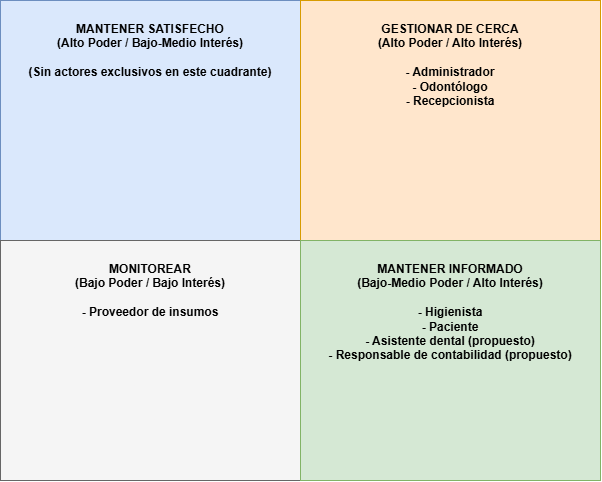
\includegraphics[width=0.88\textwidth]{figuras/matriz_poder_interes.png}
\caption{Matriz Poder-Inter\'es de las partes interesadas del sistema DentiTech.}
\label{fig:matriz_poder_interes}
\end{figure}

La clasificaci\'on de los dos roles complementarios es preliminar y deber\'a validarse con la cl\'inica. La imagen actual de la matriz representa seis roles y requiere actualizaci\'on para reflejar esta propuesta.

La distribuci\'on resultante orienta la estrategia de participaci\'on durante la ingenier\'ia de requisitos:

\begin{itemize}
    \item \textbf{Gestionar de cerca (Alto Poder / Alto Inter\'es):} Agrupa al \textbf{Administrador}, al \textbf{Odont\'ologo} y a la \textbf{Recepcionista}. Estos roles definen las reglas operativas, cl\'inicas y administrativas de la Cl\'inica Odontol\'ogica Medicus; su validaci\'on continua es indispensable para aprobar los entregables del sistema.
    \item \textbf{Mantener satisfecho (Alto Poder / Bajo-Medio Inter\'es):} No registra actores exclusivos en este cuadrante, dado que los roles con mayor capacidad de decisi\'on en la cl\'inica participan directamente en la operaci\'on diaria del sistema.
    \item \textbf{Mantener informado (Bajo-Medio Poder / Alto Inter\'es):} Comprende al \textbf{Higienista}, al \textbf{Paciente}, al \textbf{Asistente dental} y al \textbf{Responsable de contabilidad}. Sus necesidades sobre flujos de preparaci\'on cl\'inica, bioseguridad, recordatorios, claridad en presupuestos y seguimiento de cobros se recogen mediante instrumentos focalizados sin sobrecargar las decisiones arquitect\'onicas.
    \item \textbf{Monitorear (Bajo Poder / Bajo Inter\'es):} Corresponde al \textbf{Proveedor de insumos}, cuya interacci\'on se limita al intercambio est\'andar de cat\'alogos, lotes, fechas de caducidad y \'ordenes de reposici\'on.
\end{itemize}

% NOTA DE INTEGRACION: la imagen de la matriz debe actualizarse para mostrar ocho roles.

\subsection{Contexto y L\'imites del Sistema}

Siguiendo los principios de delimitaci\'on de contexto establecidos por Pohl \cite{pohl2025} y el programa de estudios IREB \cite{ireb2026}, el diagrama de contexto de la Figura~\ref{fig:diagrama_contexto} establece la frontera entre \textbf{DentiTech} y las ocho entidades externas propuestas de su entorno operativo en la Cl\'inica Odontol\'ogica Medicus.

\begin{figure}[htbp]
\centering
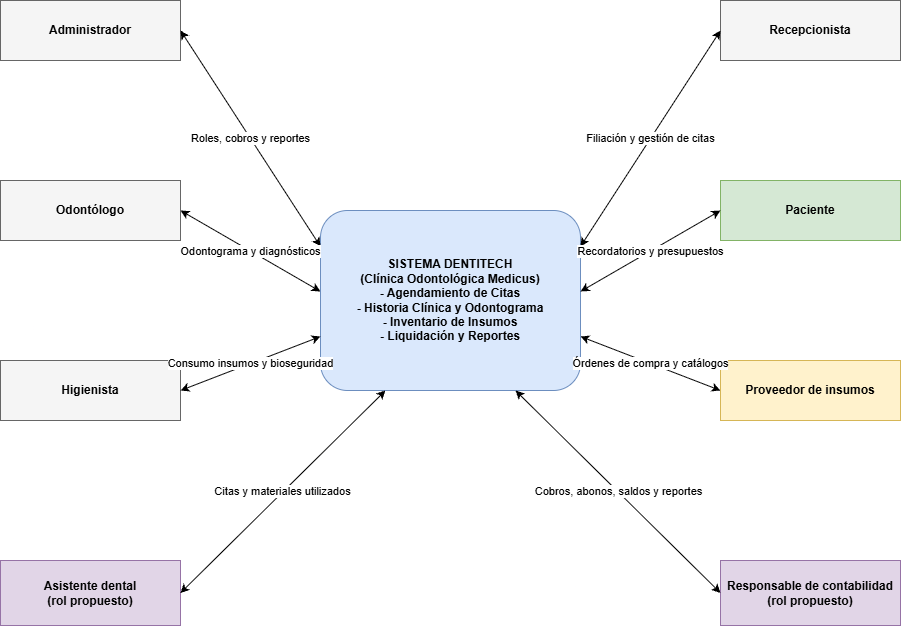
\includegraphics[width=0.95\textwidth]{figuras/diagrama_contexto.png}
\caption{Diagrama de contexto del sistema DentiTech y flujos de informaci\'on con entidades externas.}
\label{fig:diagrama_contexto}
\end{figure}

% NOTA DE INTEGRACION: actualizar el diagrama de contexto editable y su PNG
% para representar las interacciones de los dos roles complementarios.

En el modelo de ocho actores, el Asistente dental se relaciona con la consulta de citas y el registro de materiales utilizados, mientras que el Responsable de contabilidad se relaciona con la consulta de cobros, abonos, saldos y reportes. Estas interacciones se proponen para validaci\'on.

El sistema central gestiona de manera integrada el agendamiento de citas, la historia cl\'inica odontol\'ogica (odontograma, diagn\'osticos y evoluciones), el control de inventario de insumos y la administraci\'on de cobros y reportes. Quedan fuera de la frontera del software los equipos m\'edicos de diagn\'ostico por imagen (rayos X intraorales) y las plataformas bancarias externas, con las cuales \'unicamente se registran referencias documentales de resultados o comprobantes de pago.

El diagrama de contexto incluido se conserva como evidencia del modelo original de seis actores elaborado por Landy. La versi\'on gr\'afica de ocho actores est\'a pendiente de actualizaci\'on.

\subsection{An\'alisis de las Ocho Perspectivas del Contexto}

Para asegurar una comprensi\'on integral del entorno donde operar\'a \textbf{DentiTech} en la Cl\'inica Odontol\'ogica Medicus (sector Cooperativa Jet, Quevedo), la Tabla~\ref{tab:ocho_perspectivas} sistematiza el an\'alisis bajo las ocho perspectivas del contexto definidas en el s\'ilabo de la asignatura \cite{ireb2026}.

\begin{table}[htbp]
\centering
\caption{An\'alisis del entorno operativo de la Cl\'inica Odontol\'ogica Medicus seg\'un las ocho perspectivas del contexto.}
\label{tab:ocho_perspectivas}
\scriptsize
\setlength{\tabcolsep}{4pt}
\renewcommand{\arraystretch}{1.25}
\begin{tabularx}{\textwidth}{|p{2.6cm}|X|X|}
\hline
\textbf{Perspectiva} & \textbf{Aspecto Evaluado en el Dominio Odontol\'ogico} & \textbf{Hallazgo en la Cl\'inica Odontol\'ogica Medicus} \\
\hline
1. Negocio / Organizacional & Estructura jer\'arquica, flujo de atenci\'on al paciente, horarios de consulta y modelo de cobro por procedimientos. & La cl\'inica opera en el sector Cooperativa Jet de Quevedo brindando atenci\'on odontol\'ogica bajo esquema de citas programadas y atenci\'on por demanda, con cobros por sesi\'on o abonos por tratamiento supervisados por el Administrador. \\
\hline
2. Usuario / Operativa & Nivel de alfabetizaci\'on digital del personal (Administrador, Odont\'ologo, Higienista, Recepcionista) y carga en horas pico. & El personal cl\'inico y administrativo maneja herramientas ofim\'aticas b\'asicas; el registro actual de citas y fichas presenta cuellos de botella en horas de mayor afluencia de pacientes. \\
\hline
3. T\'ecnica / Tecnol\'ogica & Equipamiento de c\'omputo disponible en recepci\'on y consultorios, conectividad a internet y respaldos locales. & El establecimiento cuenta con estaciones de c\'omputo en \'area administrativa y acceso a internet comercial estable, sin un sistema integrado especializado en gesti\'on odontol\'ogica. \\
\hline
4. Datos / Informaci\'on & Volumen de historias cl\'inicas activas, estructura del odontograma, trazabilidad de abonos e inventario de insumos. & Las historias cl\'inicas, odontogramas, pagos y movimientos de insumos requieren centralizaci\'on digital para evitar duplicidad de fichas y facilitar el seguimiento hist\'orico por paciente. \\
\hline
5. Legal / Normativa & Cumplimiento de la LOPDP del Ecuador \cite{lopdp2021} respecto a datos sensibles de salud, consentimiento informado y normativa sanitaria del MSP. & La cl\'inica requiere custodia estricta de historias cl\'inicas y consentimientos informados firmados antes de intervenciones invasivas, bajo principios de confidencialidad y control de acceso por rol. \\
\hline
6. Econ\'omica / Financiera & Restricciones presupuestarias para licenciamiento de software, costos de mantenimiento e impacto de insumos caducados. & Se prioriza una soluci\'on sostenible sin costos elevados de licenciamiento recurrente, orientada a reducir p\'erdidas por caducidad de materiales entregados por el Proveedor de insumos. \\
\hline
7. Cultural / Social & H\'abitos de comunicaci\'on de los pacientes de Quevedo (preferencia por mensajer\'ia instant\'anea) y adopci\'on del sistema. & Los pacientes del sector prefieren confirmaciones y recordatorios \'agiles mediante mensajer\'ia instant\'anea, mientras que el equipo cl\'inico demanda interfaces intuitivas de r\'apida adopci\'on. \\
\hline
8. Ambiental / F\'isica & Condiciones f\'isicas de los consultorios (iluminaci\'on, bioseguridad, uso de guantes durante la consulta) que condicionan la operaci\'on. & La operaci\'on cl\'inica del Odont\'ologo e Higienista exige interfaces de registro r\'apido con m\'inima manipulaci\'on de perif\'ericos durante la atenci\'on y equipos fuera de zonas h\'umedas. \\
\hline
\end{tabularx}
\end{table}
